
%\section{User training}

Subjects were set to train their understanding of making distinguishable hand movements, using the user training GUI, where training interface corresponding to the assigned group were presented. Prior to training subjects were informed of the importance of their efforts in relation to the experiment with the intent of encourage enthusiasm. \\

The user training interface contained the following feedback: an illustration of the movement needed to
be performed, a horizontal bar visualizing the contraction level and a vertical bar plot visualizing which
movement is being recognized by the control system, as shown in \figref{fig:feedbackGUI} The only difference between control and test group was the type of confidence feedback shown trough the vertical bar plot. The test group were shown the classifier confidence scores for multiple classes thereby enabling possibility of having multiple vertical plots shown, and to correct the movement according to feedback. The control group had only the movement with the highest confidence shown thereby limiting the confidence feedback. Thus, the control group was not informed on the exact probabilities of which movements the control system recognized.      

\begin{figure}[H] 
	\centering
	\subfigure[Test group user training interface.]
	{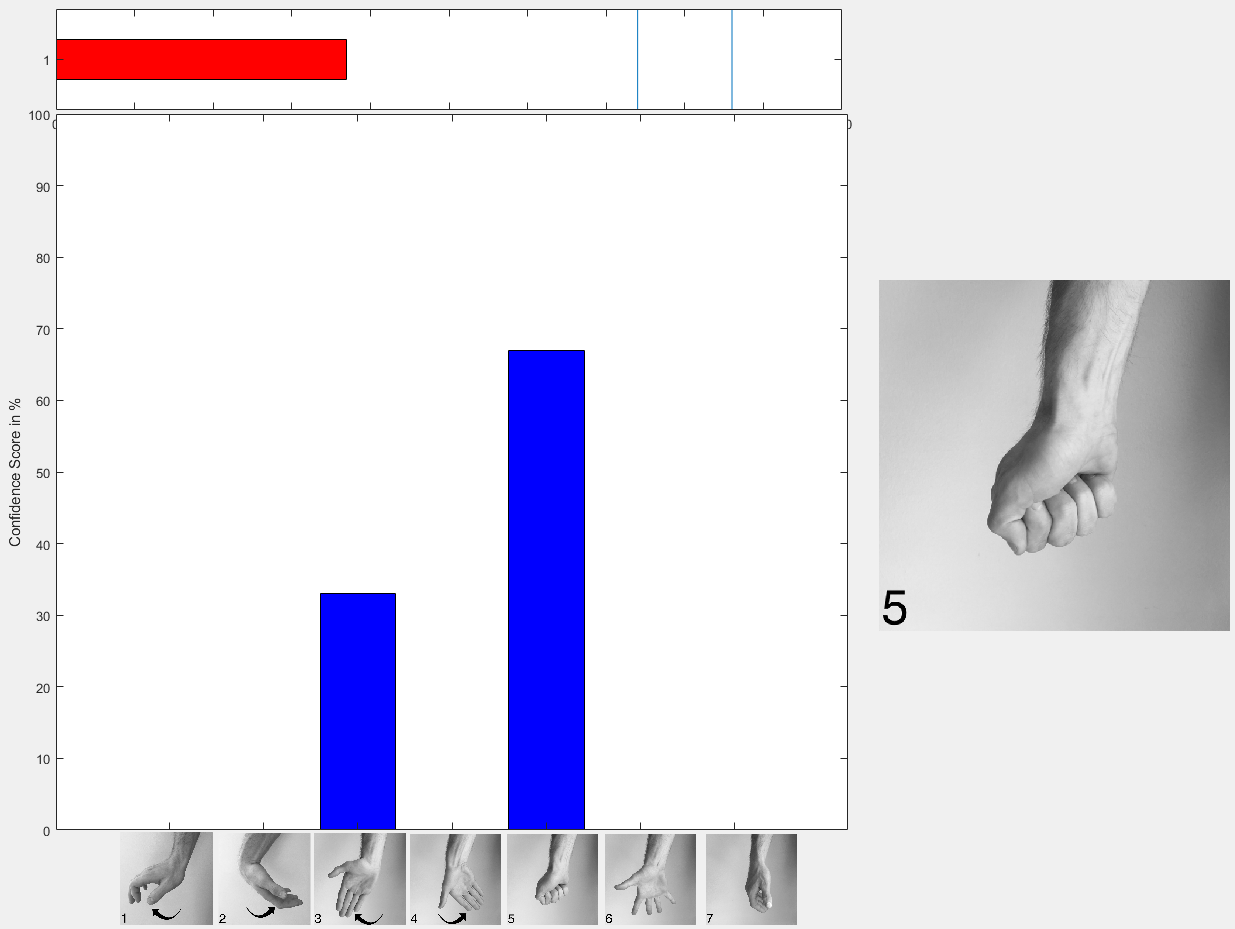
\includegraphics[width=.42\textwidth]{figures/xBackground/usertraintestGUI}} \\
	\subfigure[Control group user training interface.]
	{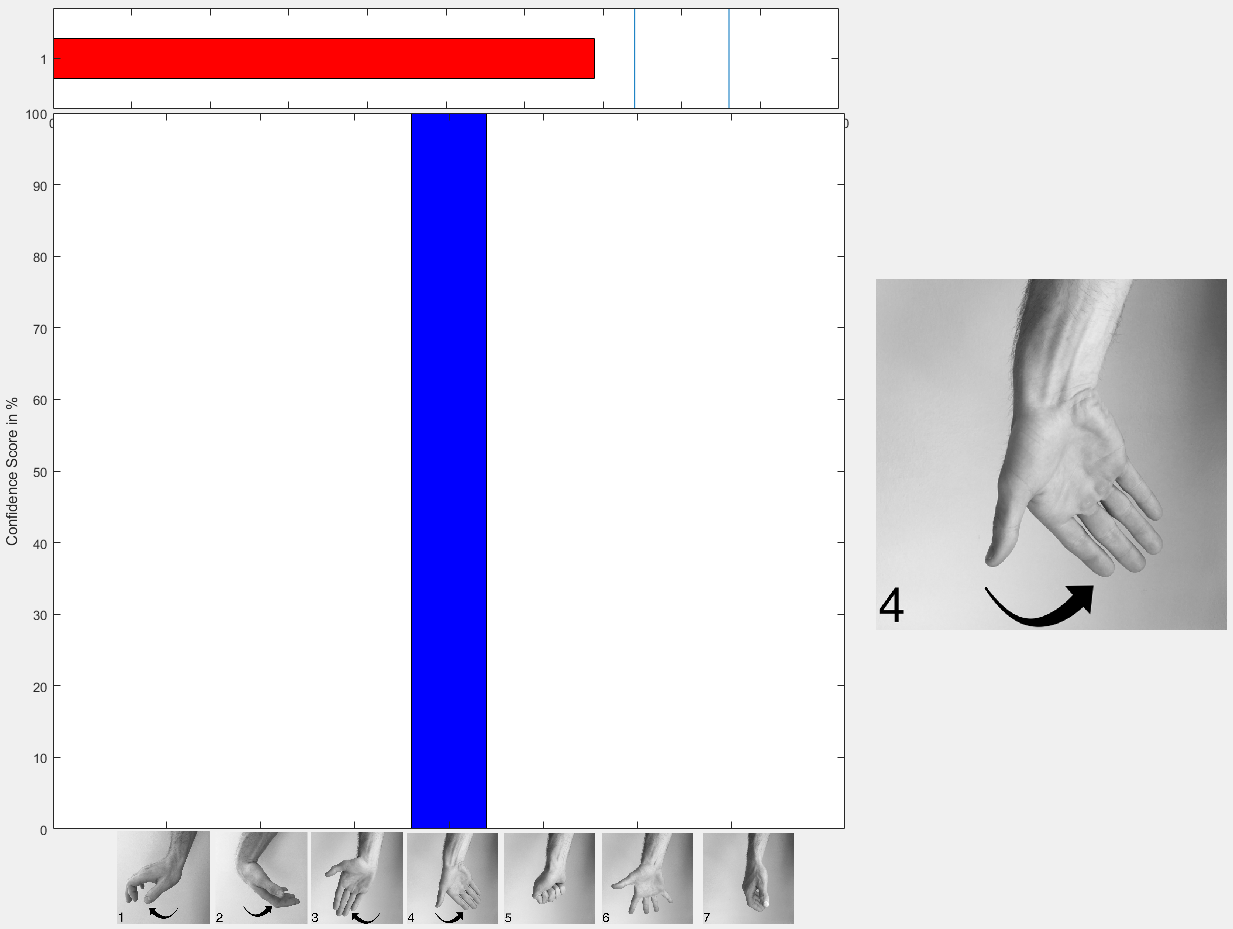
\includegraphics[width=.42\textwidth]{figures/xBackground/usertraincontrolGUI}}  
	\caption{Illustration of the user training interface for the test group (a) and the control group (b). The vertical bar plot indicates which movement is being recognized indicated by the images of each movement and the horizontal bar plot indicates contraction level. The two vertical lines in the contraction level bar plot illustrates the contraction level interval the subject must reach. The large picture of a movement on the right of the bar plot indicates which movement needs to be performed. The difference between the feedback the two subject groups receive is the information given in the vertical recognition bar plot. The control group only sees a full bar of the movement the control system recognizes the most, whereas the test groups receives the exact recognition probabilities of all movements.}
	\label{fig:feedbackGUI}
\end{figure}

The intent of user training was to train the subject in being more aware of how to perform a movement in a way the classifier would clearly recognize. Subject training were assembled as the subject had to perform the shown movement on the right side of the screen and achieve a minimum of 75\% confidence, whilst also managing to perform the movement with indicated by the boundaries in the horizontal bar plot. Once these requirements were met and withhold for one second, a sound would be played indicating task completion. The subjects had to return to the rest class and then repeat the movement. The goal was to manage as many repetitions as possible within 30 seconds, then a 10 second break was issued before moving to next movement. \\
The sequence of a training session were put together as the subject had to perform each of the six movements in combination with four different contraction level intervals; 75-85 \%, 55-65 \%, 35-45 \% and 15-25 \% of their maximum voluntary contraction (MVC), where the contraction level normalized according to their MVC. The instructed movements were trained in a random order and the subjects needed to perform all movements in the same contraction level interval before moving to a new interval. This resulted in a total training session time of 16 minutes.         


